%% $RCSfile: proj_report_outline.tex,v $
%% $Revision: 1.3 $
%% $Date: 2016/06/10 03:41:54 $
%% $Author: kevin $

\documentclass[11pt, a4paper, oneside]{report}


\usepackage{float} % lets you have non-floating floats
\usepackage{url} % for typesetting urls
\usepackage{hyperref}
\usepackage{wrapfig}
\usepackage{amsmath}
\usepackage{graphicx}

\usepackage[image,ecs]{vuwproject}

% \renewcommand{\thesection}{\arabic{section}}
% \setlength{\parskip}{\baselineskip}
\setlength{\parindent}{0pt}

%
%  We don't want figures to float so we define
%
\newfloat{fig}{thp}{lof}[chapter]
\floatname{fig}{Figure}
\graphicspath{ {./Figures/} }

%% These are standard LaTeX definitions for the document
%%                            
\title{Self Tuning Buck Converter}
\author{Niels Clayton}

\supervisors{Daniel Burmester and Ramesh Rayudu}
\otherdegree{Bachelor of Engineering with Honours}

\date{}

\begin{document}

\frontmatter

%%%%%%%%%%%%%%%%%%%%%%%%%%%%%%%%%%%%%%%%%%%%%%%%%%%%%%%

\begin{abstract}

Put in an abstract once the full report has been written.

\end{abstract}

%%%%%%%%%%%%%%%%%%%%%%%%%%%%%%%%%%%%%%%%%%%%%%%%%%%%%%%

\maketitle


% \chapter*{Acknowledgments}\label{C:ack} 
Thank you Danny B for being great :- ) 

Thank you ECS Techs for putting up with my questions 

And thank you to my wonderful girlfriend for not kicking me out when I was working on this stupid fucking project really late 

% \listof{fig}{figures}
\tableofcontents

%%%%%%%%%%%%%%%%%%%%%%%%%%%%%%%%%%%%%%%%%%%%%%%%%%%%%%%

\mainmatter

%%%%%%%%%%%%%%%%%%%%%%%%%%%%%%%%%%%%%%%%%%%%%%%%%%%%%%%

% individual chapters included here
\chapter{Introduction}\label{C:intro}

Historically power distribution has been primarily in the form of AC (Alternating current). This is credited to the fact that AC power is more efficient to transmit over long distances and made it easy to step up and down the voltages efficiently with transformers \cite{Earley2013}. However, with the invention of solid-state electronics such as the metal–oxide–semiconductor field-effect transistor or MOSFET for short, it has become possible to efficiently step up and step down direct current (DC) voltages. This has been achieved by the invention of the switch-mode power supply, which has facilitated the continued reduction of size and increase in efficiency of electronics \cite{Bocock}.

Today, switch-mode power supplies can be found in a wide variety of consumer and professional electronics, with some examples being laptops, phones, and any form of DC charger. Their widespread usage when compared to other DC-DC converters such as linear regulators can be attributed to their far greater efficiency. One such switch-mode power supply is the buck converter, which will step down a DC input voltage to a lower DC output voltage.

\section{Project Motivation}

Although buck converters are a widespread technology, they are not without their limitations and drawbacks. The current buck converter design process requires that a specific output filter be designed around the switching frequency of the converter, and the desired inductor ripple current. This filter design process will often result in the converter requiring discrete passive components that are non-standard and hard to source. This will usually result in the designer having to make compromises in their design for either the cost or the performance of the converter.

Another drawback of this design process is the static nature of both the filter and the switching components once they have been selected. This results in the buck converters desired inductor current ripple only being achieved at a very specific designed output voltage or load. This means that with current buck converter designs varying the desired output voltage or varying the output load will cause the inductor current ripple to vary. This is an issue, as very few loads are static and will not change during their operation. 

\section{Project Goals}\label{S:goals}

The goal of this project is to develop a testing platform through which the effects of variable buck converter switching frequency on inductor current ripple can be observed and controlled. The aim of this is to eliminate the need to design the output stage of the buck converter by implementing a control system to maintain a specified inductor current ripple, and output voltage.

To achieve this goal, a proof of concept buck converter will be designed to operate as the testing platform. This converter will require a variable frequency pulse width modulated (PWM) signal generator, and inductor current ripple sensing. This will allow for direct manipulation and control of inductor current ripple. The converter will also need to implement the full functionality of existing buck converter designs, including controlled output voltage regulation.\\

The following list of specifications outlines the requirements the designed test platform will meet:

\begin{itemize}
    \item Operate with a 12V DC input supply voltage
    \item Provide a selectable DC output voltage between 3V and 10V
    \item Provide an output voltage precision of at least $\pm5\%$
    \item Be capable of varying the the converters switching frequency between 1$k$Hz and 100$k$Hz
\end{itemize}

% This project aims to eliminate the need to design the output stage of a buck converter. By implementing a control system that varies the switching frequency of the converter, we will be able to directly manipulate the inductor current ripple. This project aims to produce a proof of concept buck converter that is capable of operating at 12V, with an output range of 3-10V and precision of $\pm5\%$. The converter will also be able vary its switching frequency between 1$kHz$ and 100$kHz$, allowing for selection of inductor current ripple between 20\% and 50\% with precision of $\pm5\%$. All of this must be implemented while maintaining the standard functionality of the converter.


% \subsubsection{TODO Expand on the project goals, possibly convert the previous section into a bulleted list of project goals and requirements.}

% This will be referenced in the implementation and design sections many times, so it needs to clearly outline what we are looking to achieve in this project. 
\chapter{Background}\label{C:background}

A literature research was performed to inform design decision made in this project, and to evaluate any existing research. It will discuss buck converter design factors and topologies, as well as the various different methods of PWM generation. In performing this literature research, we searched Google Scholar, Engineering Village, and Te Waharoa to find designs that utilised variable frequency PWM. 

These searches returned no research relevant to the designs of this project, with the only related work focusing on the electromagnetic noise reduction using randomised frequency modulation \cite{Roman2001,Familiant2016}. Because of this, research was instead performed to inform the design of the buck converter and the generation of PWM signals.

\section{Pulse Width Modulated Signal Generation}\label{S:PWM_back}

Pulse width modulation (PWM) is a digital signal generation technique shown in \Cref{F:PWM}, in which the Period $T$ of the signal is held constant, while the ratio of its logic high period $T_{on}$ to logic low period $T_{off}$ is modulated. This ratio of high period to the low period is referred to as the duty cycle of the PWM signal and is often expressed as a percentage, this can be seen in \Cref{F:Duty}.\\

PWM signals are used in a wide variety of applications for both digital and analogue electronics. PWM is often used to generate analogue signals from digital components by varying the average voltage of the digital PWM signal over time \cite{Tareen2019}. PWM is also used to control the switching elements contained within switch mode power supplies using this same principle, as discussed in \Cref{S:buck_back}. With regard to this project, we will be looking to generate a PWM signal that can be modulated in both duty cycle and frequency.

\begin{figure}[H]
      \centering
      \begin{subfigure}{0.45\textwidth}
          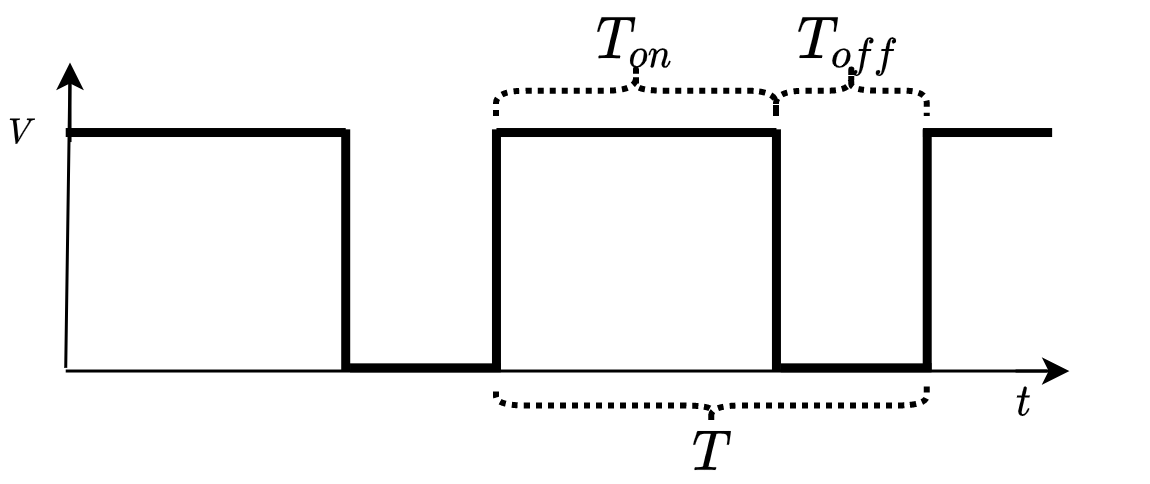
\includegraphics[width=\columnwidth]{PWM.png}
          \subcaption{Pulse width modulated signal}
          \label{F:PWM}
      \end{subfigure}
      \hspace{10pt}
      \begin{subfigure}{0.5\textwidth}
          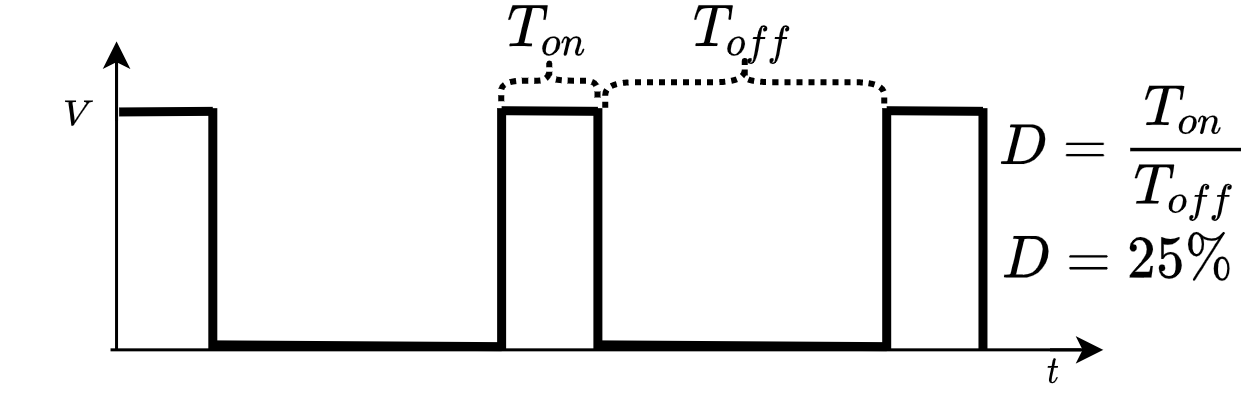
\includegraphics[width=\columnwidth]{Duty_cycle.png}
          \vspace{-6pt}
          \subcaption{Duty cycle calculation}
          \label{F:Duty}
      \end{subfigure}
      \caption{Pulse width modulated signal characteristics}
      \label{F:PWM_description}
  \end{figure}

\subsection{Analogue PWM Signal Generation} \label{S:analogue_PWM_back}

Designing a PWM signal generator using analogue components has three distinct stages required to generate the signal. These stages can be seen in \Cref{F:analogue_PWM}, and include clock generation, triangle wave generation, and signal comparator stages \cite{Caldwell2013}.\\ 

The clock generation stage generates a square wave clock signal at a set frequency. This is usually done using a quartz crystal oscillator, or another form of resonating oscillator circuit. The triangle wave generating state must take the clock signal from the previous stage, and produce a triangle wave of the same frequency. This stage is most often done using a standard op-amp integrating circuit with unity gain at the resonating frequency of the clock source. The final signal comparator stage will convert this triangle wave into a PWM signal. Using a comparator, a refrence voltage can be applied to the non-inverting input, and then the triangle wave can be applied to the inverting input. This will produce a pulse train with the same frequency as the clock source, where the period of $T_{on}$ and $T_{off}$ is set by the refrence voltage. 

\begin{figure}[H]
	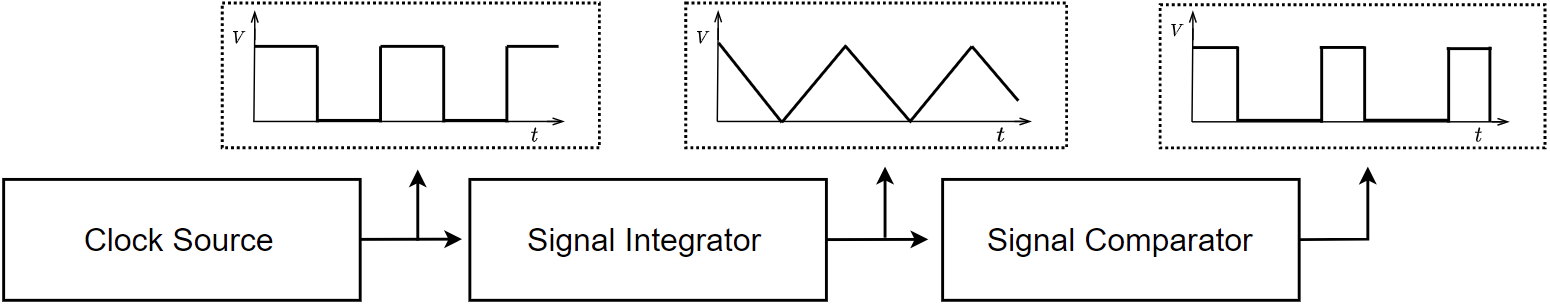
\includegraphics[width = 1\textwidth]{Analogue_PWM.png}
	\caption{Stages of analogue PWM generation}
	\label{F:analogue_PWM}
\end{figure}


\subsection{Digital PWM Signal Generation}\label{S:digital_PWM_back}

Designing a PWM signal generator with digital components is far simpler than the method described in \Cref{S:analogue_PWM_back}, and can be done using either a microcontroller or a Field Programable Gate Array (FPGA). By using an internal timer that is continually incrementing at a known period we can set a period for our PWM. Then by toggling a digital I/O when a compare variable is equal to the value of the timer. we are able to generate a PWM signal with a variable duty cycle \cite{Colley2020}. This can be achieved on most microcontrollers, however the maximum frequency and duty cycle accuracy will be dependant on individual clock speed and internal register sizes.

\section{Buck Converters}\label{S:buck_back}

The buck converters is a variant of a switch mode power supply that steps down a DC input voltage to a DC output voltage. They are commonly used in a wide variety of consumer and professional appliances such as laptops, phones, and chargers due to their high efficiency compared to other DC-to-DC step down converters such as linear regulators \cite{Mohan2012}.\\

The basic operational components of a buck converter can be seen below in \Cref{F:buck_func}. From this we see that a buck converter has three main elements, the input voltage source, two switching components, and an output filter across the load. In the case of \Cref{F:buck_func}, the first switching component is an actively controlled switch such as a MOSFET or transistor, and the second a passive switching diode. This configuration of an active and a passive switch is known as the non-synchronous buck converter topology, if the passive diode were to be replaced with a second active switch the topology would be considered synchronous. Although both topologies function under the same fundamental principles, the non-synchronous topology is easier to implement with the drawback of higher losses and therefor lower efficiency.\\

It can also be seen from \Cref{F:buck_func} that a buck converter has two operating states that are controlled through the activation of these switching components. By toggling these switching components at high speed though the use of PWM, we can control the current flowing through the inductor of the output filter. By controlling this current we are also able to directly control the current through, and voltage across the output load of the converter. Using this, buck converters will often have a feedback control system in their design to be able to actively control and regulate the output voltage during usage. This controller will vary the duty cycle of the the switching PWM signal, thereby varying the output voltage of the buck converter as shown in \Cref{E:V_out}.\\

\begin{figure}[H]
	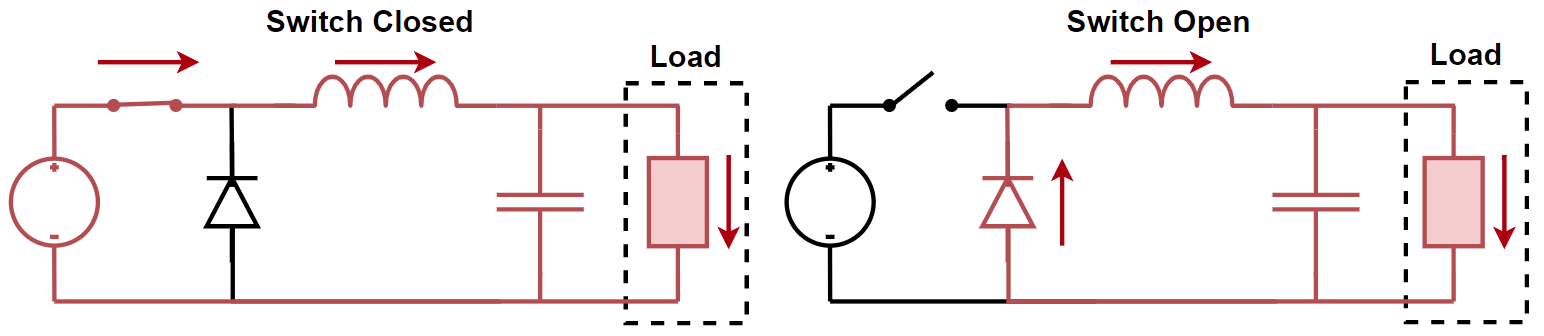
\includegraphics[width = 1\textwidth]{Buck_Functionality.png}
	\caption{Operating states of a buck converter}
	\label{F:buck_func}
\end{figure}


\subsection{Buck Converter Design}\label{S:buck_design_back}

The design of a common buck converter has two primary considerations, the output voltage of the converter $V_0$, and the inductor current ripple of the converter $\Delta i_L$. These considerations can be specified by designing the buck converter using \Cref{E:V_out} \& \Cref{E:delta_i} \cite{Mohan2012_Design,Hauke2015}.\\ 

When designing a buck converter the first design specification that must be met is the output voltage. In \Cref{E:V_out} the output voltage can be directly related to the input voltage $V_{in}$ and the switching duty cycle $D$. Using this equation it is possible to directly set the output voltage of the buck converter by varying this duty cycle.

\begin{align}\label{E:V_out}
	V_o &= D \cdot V_{in}
\end{align}

Once the output voltage has been specified, the inductor current ripple can be calculated and specified with \Cref{E:delta_i}. This equation allows for the inductor current ripple to be directly related to the inductor size $L$, and the PWM switching frequency $f_s$. This allows the the specification of the inductor current ripple through the varying of these two values.

\begin{align}\label{E:delta_i}
   \Delta i_L &= \frac{ V_{o} \cdot \left( 1 - D \right) } {L \cdot f_s}
\end{align}

These two equations will be used to inform the designs and specifications of this project, and will be discussed in detail in \Cref{S:specs}.




\section{Current Sensing}\label{S:current_sense_back}

Discuss the varying methods of current sensing that are available, and what each of their advantages and disadvantages are.

\subsection{Hall Effect Sensors}\label{S:hall_effect_back}

brief overview of hall effect sensors. They function by measuring the magnetic flux density, meaning that they are commonly used to senses the presence of a magnet. However since a current flowing though a wire will produce a magnetic flux, they can also be used to measure current flow.

Because of this operation, they are able to sense a current without contacting or altering the circuit. This means that they are commonly used in the measurement of high voltage or high current circuits, as they will remain completely isolated from the circuit being sensed, and will also not dissipate power from the sensed circuit. This provides large safety advantages, and can often decrease the complexity of the sensing circuit. 

Hall affect sensors do however suffer from a lack of precision. Due to their operation, their measurements will constantly be offset by any ambient magnetic flux. This means that they are not commonly used for the sensing of small signal currents, as the noise floor of the Earths own magnetic field can often be larger than the signal being sensed.  


\subsection{Current Sense Amplification}\label{S:current_shunt_back}

Current sense amplification works on the basic principle of Ohm's law $I=\frac{V}{R}$. By sensing the voltage dropped across a known value resistive element (Often called the current shunt), it is possible to calculate the current that is flowing through the element. This form of current sensing is very simple to implement in theory, however it has the effect of altering the system being sensed by adding a resistive load, and thereby increasing the losses of the system. 

To mitigate the effects of this sensing on a circuit, a smaller resistive load can be used. However, this will also decrease the measurable voltage across the load, and therefore decrease the precision of a taken measurement. Because of this, shunt based current sensors are often paired with an operational amplifier known gain. This combination allows for accurate amplification of the shunt voltage drop, increasing the precision of the measurement, and allowing for drastically smaller shunt resistors. 




\section{Control Systems}\label{S:control_back}

Discuss the basics of control theory, and how a controller can be implemented on a digital system within discrete time. 

\begin{itemize}

    \item
        Discuss in very general terms what a control system is what what it seeks to do in a system.

    \item
        Discuss what the control system will be doing in the case of this project. Talk about how a controller will be used to control both the output voltage of the converter, and the inductor ripple of the converter.

    \item 
        Discuss the design, use, and implementation of a PID controller within a system. 

\end{itemize}

\subsection{PID Controllers}\label{S:PID_back}
\chapter{Work Completed}\label{C:work}

This chapter will discuss the work that has been completed so far on this project. It will begin by discussing the projects requirements', using them to design and justify the final specifications of the system. Once the specifications are outlined, the architecture and design of the final system will be discussed. Finally the design and current implementation of the PWM signal generator will be specified.  

\section{Defining \& Justifying System Specifications}\label{S:specs}

Based on the system requirements that have been outlined in \Cref{C:intro}, a set of system specifications can be created to inform the design. Current work on this project has been towards the implementation of the PWM signal generator, and as such all specifications outlined will pertain to this work.

The final system is required to be able to select both the output voltage and inductor current ripple of the buck converter. From this requirement we specify that our PWM generator must vary both the duty cycle and the switching frequency of the buck converter, based on \Cref{E:V_out} \& \Cref{E:delta_i}. The requirements also specify the level of precision that will be required for these selections, allowing us to specify the tolerable error. Using these same equations, the minimum duty cycle step size in \Cref{E:duty_step}, the inductor minimum and maximum values in \Cref{E:L_min} \& \Cref{E:L_max}, and the frequency step size in \Cref{E:f_step} have all been derived. For the derivation of these values see \Cref*{A:specs}.\\

Duty cycle step calculation:
\begin{align}
    V_{error} &= V_{min} \cdot error = 0.15V\\
    D_{step} &= \frac{V_{error}}{V_{in}} = 0.0125\\
    N_{step} &= \frac{1}{D_{step}} = 80 \label{E:duty_step}
\end{align}

Inductor Sizing Calculations:
\begin{align}
    L_{max}&=\frac{V_{max}\cdot\left(1-D_{max}\right)}{f_{min}\cdot I_{min}} = 27.7mH \label{E:L_max}\\ 
    L_{min}&=\frac{\frac{V_{in}}{2}\cdot\left(1-0.5\right)}{f_{max}\cdot I_{min}} = 0.5mH \label{E:L_min}
\end{align}

Frequency step calculation:
\begin{align}
    f_{step}&=\frac{V_{max}\cdot\left(1-D_{max}\right)}{\left(I_{min}-I_{Error}\right)\cdot L_{max}}-f_{min} = 52Hz\\
    N_{steps}&=\frac{\left(f_{max}-f_{min}\right)}{f_{step}} = 1881 \label{E:f_step}
\end{align}

From these equations we can build a list of final specifications to inform the design of our PWM generator and buck converter. The PWM generator must provide a minimum voltage step size of $0.0125V$, for a resolution of 80 voltage steps between 3V and 10V. The PWM generator must also be able to provide a minimum frequency step size of $52Hz$, for a resolution of 1881 frequency steps between $1KHz$ \& $100kHz$. Finally we can also specify that the buck converter must be capable of functioning with inductor values between $0.5mH$ \& $27.7mH$. \\

By designing the PWM generator and the buck converter to these specifications, we are able to guarantee that we can always achieve the requirements outlined in \Cref{C:intro}.

\section{System Architecture \& Design}\label{S:system}

To achieve the specifications that have been outlined in \Cref{S:specs}, it is important to design the system architecture around them. In \Cref{F:sys_overview} an overview of the system architecture can be seen, with three main design sections outlined. These sections each represent a significant segment of work that must be completed for the final artefact of this project to be achieved. \\

The first section of work that must be completed is the design of the PWM generation, denoted 1 in \Cref{F:sys_overview}. This PWM generator will be used to control both the output voltage and the inductor current ripple, and as such must be able to modulate both the duty cycle and the frequency of the PWM to the precisions required. \\

The second section of work is the design of the sensing elements required by the system, denoted 2 in \Cref{F:sys_overview}. These elements will be used to measure both the output voltage and the inductor current ripple, and therefor must be able to achieve the required precisions and sampling rates. \\

Finally the third section of work is the design and implementation of the two control systems, denoted 3 in \Cref{F:sys_overview}. These control systems will be responsible for maintaining the desired output voltage and inductor current ripple of the buck converter. This system will therefor be responsible for facilitating the final functionality of the project, combining sections 1 \& 2. \\

\begin{figure}[!h]
    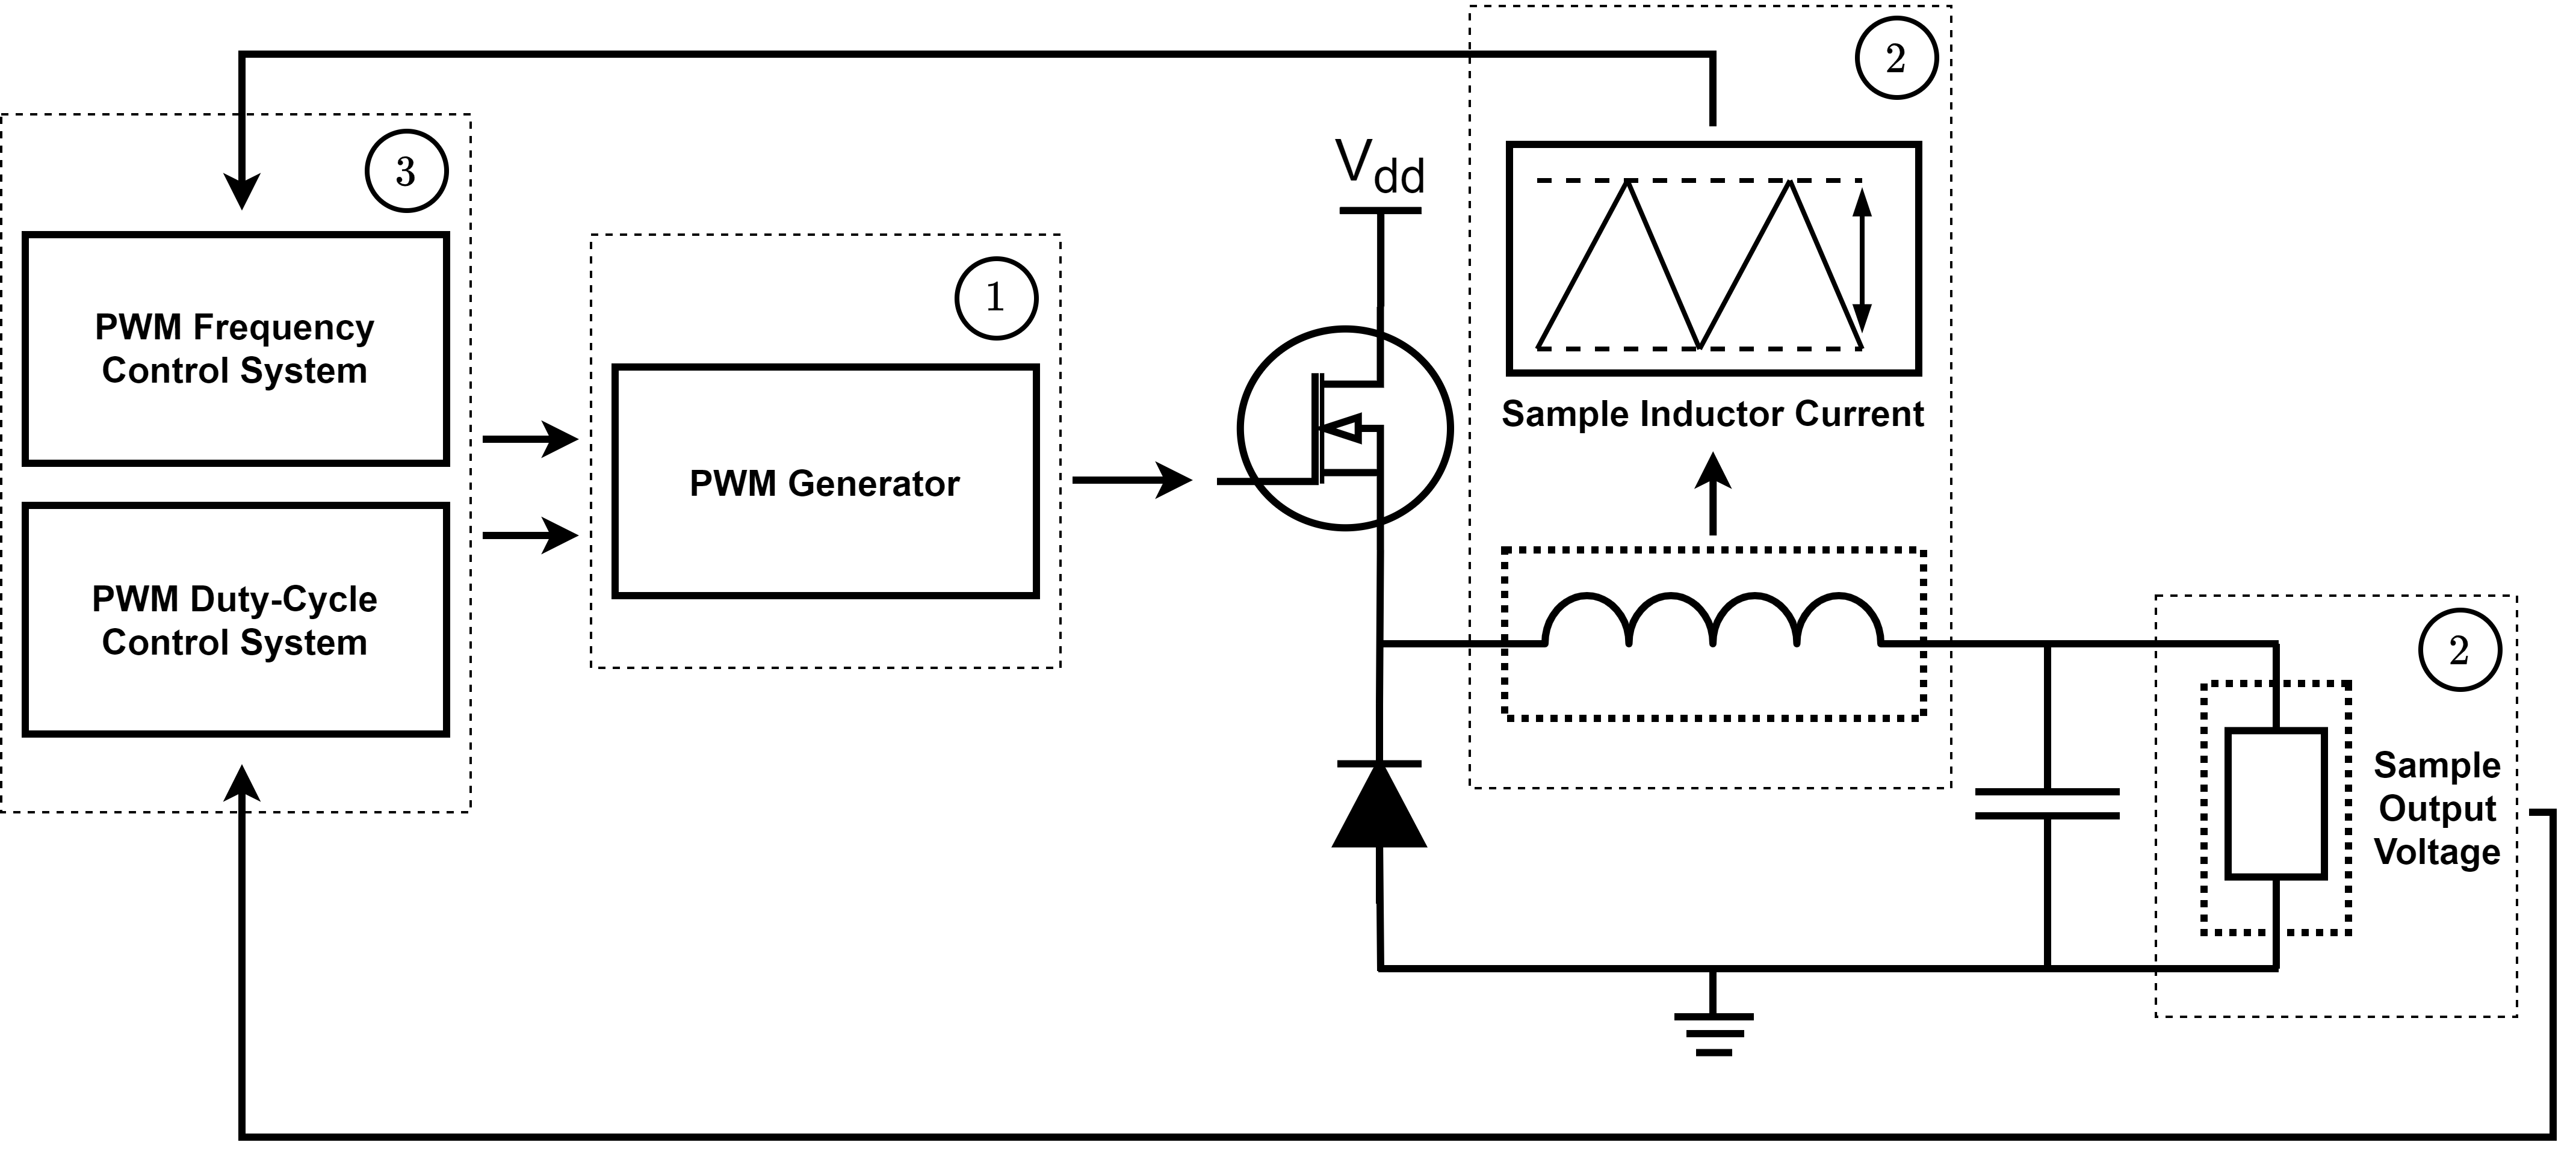
\includegraphics[width = 0.95\textwidth]{System_Overview.png}
    \caption{High level system overview}
    \vspace{-20pt}
    \label{F:sys_overview}
\end{figure}

\section{PWM Generation Design}\label{S:pwm_gen}

In the design of the PWM generator, both the analogue and digital designs discussed in \Cref{S:PWM} were considered, designed, and tested for. Each of these designs presented pros and cons that would affects the overall design of the system architecture. This section will discuss these designs and finalise the design of the PWM generator for this system. 

\subsection{Analogue PWM Generator Design}\label{S:analogue_design}

As discussed in \Cref{S:analogue_PWM}, the design of the analogue PWM signal generator requires three stages, each of which will have its own design requirements based on the specifications outlined in \Cref{S:specs}. \\

The clock generation stage will be responsible for setting the frequency of the final PWM signal. This specifies that the clock source have a variable frequency output range between $1kHz$ and $100kHz$, with a minimum step size of $52Hz$. Research was done on a variety of clock sources, looking at voltage-controlled oscillators (VCO's), signal generator IC's, and even the basic 555 timer. From this VCO's were identified to operate at much higher frequencies than those used in this project. It was also identified that signal generator IC's often require selections of passive components to operate effectively, increasing their complexity. For this reason the variable frequency 555 timer circuit was selected, as it provided the required specifications.\\

The next section designed was the signal integrator stage. This stage consisted of a basic op-amp integrator circuit, with a design requirement that it be able to integrate the clock signal across the frequency range required. This circuit was designed and implemented in an LTSpice simulation to evaluate it's performance, and can be seen in \Cref*{A:analogue_PWM}. From this simulation it was noted that the integrator's frequency response was similar to that of a first order low pass filter, and greatly attenuated the integrated signal. For this reason it was decided that analogue PWM generation would not be implemented in this system, as it presented many issues.

\subsection{Digital PWM Generator Design}\label{S:digital_design}

As discussed in \Cref{S:digital_PWM}, The design of the digital PWM generator is far simpler than that of the analogue, and can be implemented in a wide variety of methods. In this project microcontrollers and FPGA's have been considered.

Based solely on the capabilities of the platform, the PWM generator would be best designed and implemented on an FPGA as it would allow for superior speed and precision. However FGPA design brings a lot of difficulties, primarily in the prototyping and testing stages. Because of this, due to the limited time from of this project, we have decided to implement this PWM design using a microcontroller.

The selection of the microcontroller is highly dependant on the clock frequency and design of the PWM peripherals, as it must be capable of achieving the specifications outlined in \Cref{S:specs}. A large selection of microcontroller datasheets were reviewed to identify their specifications, including AVR, STM8, Espressif, and teensy based microcontrollers. From this review it was decided that the ESP32 microcontroller would be best suited to this project \cite{ESP32Manual}. This microcontroller is capable of outputting a maximum PWM frequency 125$kHz$ with a duty cycle resolution of 9 bits (512 voltage steps). From here a short C program was written to test the PWM functionality of the ESP32, and it was confirmed that it met the required specifications. The source code and images of this PWM signal can be found in \ref{A:digital_PWM}.
\chapter{Future Plan}\label{C:future} 

\section{Work to be Completed}

\begin{itemize}

    \item 
    Discuss what work I still have to do before beginning the evaluation of the system. 

    \begin{itemize}
        \item Select sensors to measure peak-to-peak ripple current
        \item finalise the circuit design for the project, this includes selection all other components needed for it's operation.
        \item Create a final PCB for the design 
        \item Design the controller that will control both output voltage and inductor ripple 
    \end{itemize}

\end{itemize}

\section{System Evaluation}


    The evaluation of this project will be based upon meeting the following selection of specifications. All evaluations of the design will be conducted using a 10$\Omega$ output load, with an input voltage of 12V DC.

\begin{itemize}
	\item The buck converter will be able to take input voltages up to 12V DC
	
	\item The buck converter maintains basic functionality of $V_{out} = D\times V_{in} - \mathrm{effeciency}$

	\item The buck converter will output voltages between 3V and 10V DC
	
	\item The output voltage accuracy will be within $\pm 5\%$ of the target output voltage

	\item The user will be able to define the inductor ripple between 20\% and 50\%, with increments of 5\%.
	
	\item The inductor ripple accuracy will be within $\pm 5\%$ of the defined inductor ripple
	
	\item The buck converter will have a switching frequency range of 1k$Hz$ to 100k$Hz$

\end{itemize}

\section{Project Timeline}

\begin{itemize}

    \item 
    Create another Gant chart that now more accurately breaks down the required tasks into the remaining time. Discuss this chart and why it is set out the way that it is. 

\end{itemize}



\section*{Feedback}\label{S:feedback} 

% This could highlight any difficulties currently faced, and make specific requests for guidance from the examination committee. For example, a student may be unsure how best to evaluate their artefact, and would appreciate suggestions for alternative methods. 

\begin{itemize}
    \item I want to ask for some suggestion on evaluating the final artefact. The evaluation described within my proposal has not changed, and it seems to be very simple at the moment.   
\end{itemize}
\chapter*{Feedback}\label{C:feedback} 

% This could highlight any difficulties currently faced, and make specific requests for guidance from the examination committee. For example, a student may be unsure how best to evaluate their artefact, and would appreciate suggestions for alternative methods. 

\begin{itemize}
    \item I want to ask for some suggestion on evaluating the final artefact. The evaluation described within my proposal has not changed, and it seems to be very simple at the moment.   
\end{itemize}



%%%%%%%%%%%%%%%%%%%%%%%%%%%%%%%%%%%%%%%%%%%%%%%%%%%%%%%

\backmatter

%%%%%%%%%%%%%%%%%%%%%%%%%%%%%%%%%%%%%%%%%%%%%%%%%%%%%%%


\bibliographystyle{ieeetr}
% \bibliographystyle{acm}
\bibliography{bibliography}


\end{document}
